%----------------------------------------------------------------------------
\chapter{Tesztkörnyezet}
\label{chapt:birdmap-test}
%----------------------------------------------------------------------------
Az alkalmazásom fejlesztésének megkönnyítése érdekében nagy hangsúlyt fektettem a tesztelhetőségre.
Helyettesíteni akartam az éles rendszer komponenseivel való kommunikációt,
hogy abban az esetben is folyni tudjon a fejlesztés, ha a rendszer épp nem elérhető.
Ezen kívül hasznos, ha az alkalmazás által feldolgozott adatok személyre szabhatóak,
hiszen sokszor olyan problémákra lehet így fényt deríteni, amelyek nem vagy csak jóval később jönnének elő az éles rendszer használata során.

A tesztelhetőség megvalósításához három szoftver komponenst kell helyettesítenem,
melyeket az alábbi szekciókban ismertetek.
%----------------------------------------------------------------------------
\section{Helyettesítő szolgáltatások}
%----------------------------------------------------------------------------
Az alkalmazásom szerver oldali szolgáltatásai a Birbnetes Command and Control (a kódban Device) és Input Service-ekkel azok OpenAPI leíróiból generált interfészein keresztül kommunikál.
Ezen intefészek mögé bármilyen implementáció regisztrálható, mely helyettesíti az éles rendszer működését.

Készítettem egy osztályt \verb+DummyDeviceAndInputService+ néven, mely a szerver indulásakor mű eszközadatokat generál egy lokális változóval állítható darabszámban,
majd ezeket egy belső listában tárolja. Az eszközök státuszát és koordinátáit egy véletlenszám generátor segítségével határozom meg.
Az osztály implementálja a Device Service interfészét, melynek metódusai az imént említett mű eszközlista elemeivel dolgoznak,
azok státuszát olvassák és módosítják.
Illetve implementálja az Input Service interfészét, 
melynek metódusa bármilyen paraméterből kapott egyedi azonosító esetén visszaad egy véletlenszerűen kiválasztott bekapcsolt státuszú eszközt a listából.

Az alkalmazás által regisztrált és ezáltal használt intefész implementációi a konfigurációs fájl egy logikai értéke alapján cserélhető az éles és a helyettesítő között,
a \ref{lst:dummy-service-registration}-es listában látható módon.
\newpage
\begin{lstlisting}[style=csharp, caption=A helyettesítő és az éles szolgáltatások regisztrálásának logikája, label=lst:dummy-service-registration]
    if (configuration.GetValue<bool>("UseDummyServices"))
    {
        services.AddTransient<IInputService, DummyDeviceAndInputService>();
        services.AddTransient<IDeviceService, DummyDeviceAndInputService>();
    }
    else
    {
        services.AddTransient<IInputService, LiveInputService>();
        services.AddTransient<IDeviceService, LiveDeviceService>();
    }
\end{lstlisting}


%----------------------------------------------------------------------------
\section{MQTT teszt alkalmazás}
%----------------------------------------------------------------------------
Az MQTT.NET szoftvercsomag github oldalán található néhány példa a csomag használatára \cite{mqttnet-examples}.
Ezek között találtam Sepp Penner MQTTnet.TestApp.WinForm \cite{mqttnet-winforms} projektjét, 
mely egy Windows Forms applikáció az említett szoftvercsomag által nyújtott funkcionalitások tesztelésére.
Indítható vele MQTT szerver, feliratkozó kliens és publikáló kliens is.
Ezek meglétével az alkalmazás képes az üzenetek manuális publikálására egy a felületen beállítható témában.
Én azonban szerettem volna az üzeneteket automatikusan bizonyos időközönként küldeni,
ezért átalakítottam az alkalmazást az igényeimnek megfelelően a \ref{fig:mqtt-tester}-es ábrán látható módon.
Elhelyeztem a fejlületen egy csúszkát, mellyel az üzenet küldés intervalluma állítható, illetve két új gombot,
melyekkel az üzenet küldő időzítő indítható és megállítható.
Az alkalmazás képes üzenetek adatainak generálására, mellyel az AI Service által publikált üzenetek modelljeivel azonos adatokat generálok.
\begin{figure}[!ht]
    \centering
    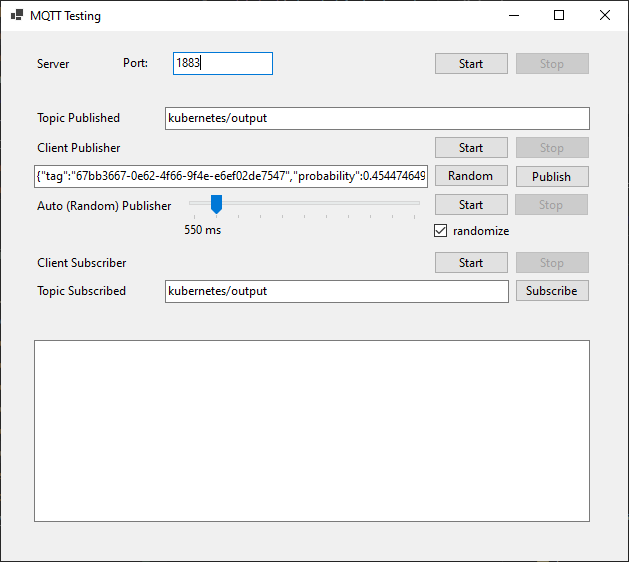
\includegraphics[width=150mm, keepaspectratio]{figures/MQTT-Tester.png}
    \caption{Az MQTT kommunikációt tesztelő alkalmazás felületének egy része}
    \label{fig:mqtt-tester}
\end{figure}
